\subsection{Motors}\label{subsec:motors}

\subsubsection{Objectives}\label{subsubsec:objectives}
We want to be to stop a ball with a velocity of maximum $7m/s$.

\subsubsection{Calculations for the moving motor}\label{subsubsec:moving_motor}
The distance from the attacker to the goal is 0.4m.
That means we have stop the ball in
\begin{equation}
    \label{eq:stopping_time}
    t = \frac{s}{v} = \frac{0.4m}{7m/s} = 0.057s
\end{equation}
Which is not a lot of time to process the image and move the motors.
The goalkeeper has to travel a maximum distance of 0.2m in 0.057s, that means we have an average velocity of
\begin{equation}
    \label{eq:average_velocity}
    v = \frac{s}{t} = \frac{0.2m}{0.057s} = 3.5m/s
\end{equation}
Which means we need a top speed of at least $2\cdot3.5m/s=7m/s$, as the motors have to accelerate and decelerate.
We also need to be able to move the motors in 0.057s, which means we need a maximum acceleration of
\begin{equation}
    \label{eq:acceleration}
    a = \frac{v}{t} = \frac{7m/s}{0.057s} = 122.8m/s^2
\end{equation}
We assume that the weight of the tubes is $\sim 0.1kg$.
The torque needed to move the tubes is
\begin{equation}
    \label{eq:torque}
    \tau = F \cdot r = m \cdot a \cdot r = 0.1kg \cdot 122.8m/s^2 \cdot 0.083m \approx 1Nm
\end{equation}
assuming the radius of the gear is 8.3m.
And the required top RPM is
\begin{equation}
    \label{eq:top_rpm}
    \text{RPM} = \frac{v}{2\pi r} \cdot 60 = \frac{7m/s}{2\pi \cdot 0.083m} \cdot 60 \approx 800\text{RPM}
\end{equation}
A Motor that fits those requirements is the \textbf{PD42-3-1141} from \textbf{Trinamic}.

\subsubsection{Calculations for the rotating motor}\label{subsubsec:rotating_motor}
The ball has a mass of 17g.
We assume that we have an angle of 45\deg  to accelerate the ball.
\\
\begin{center}
    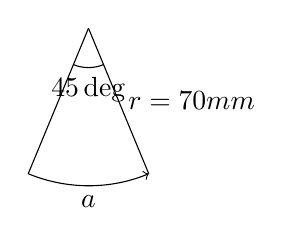
\begin{tikzpicture}
        \def \r {2}
        \def \rsmall {0.5}
        \def \angle {45}
        \draw (0,0) -- ({-sin(\angle / 2)*\r}, {-cos(\angle / 2)*\r});
        \draw (0,0) -- ({sin(\angle / 2)*\r}, {-cos(\angle / 2)*\r}) node[right, midway] {$r=70mm$};
        \draw ({-sin(\angle / 2)*\rsmall}, {-cos(\angle / 2)*\rsmall}) arc(270-\angle/2:270+\angle/2:\rsmall) node[midway,below] {$45\deg$};
        \draw[->] ({-sin(\angle / 2)*\r}, {-cos(\angle / 2)*\r}) arc(270-\angle/2:270+\angle/2:\r) node[midway,below] {$a$};
%        \draw () circle (\r);
    \end{tikzpicture}
\end{center}
%    \\
That means we have the distance $a$ to accelerate the ball.
\begin{equation}
    \label{eq:distance}
    a = r \cdot \frac{\pi}{4} = 70mm \cdot \frac{\pi}{4} = 55mm
\end{equation}
The goal is to shoot the ball back at a speed of 7m/s.
The time to accelerate the ball is
\begin{equation}
    \label{eq:time}
    t = \frac{2\pi\cdot r}{v} = \frac{2\pi\cdot 70mm}{7m/s} = \frac{\pi}{50} \approx 0.06s
\end{equation}
The maximum speed can easily be calculated with
\begin{equation}
    \label{eq:max_speed}
    \omega = \frac{60s/min}{t} = \frac{60s/min}{0.6s/rotation} = 1000\text{RPM}
\end{equation}
For the motor that just rotates the figure we can use a DC motor with gears and an encoder.
% Pololu 10:1 Metal Gearmotor 37Dx65L mm 12V with 64 CPR Encoder (Helical Pinion) 4758
A motor that fits those requirements is the \textbf{Pololu 10:1 Metal Gearmotor 37Dx65L mm 12V with 64 CPR Encoder (Helical Pinion) 4758}.

\subsection{Camera}\label{subsec:camera}

\subsubsection{Optics}\label{subsubsec:lens}

\paragraph{Lens Equation}\label{par:lens_equation}

The relationship between the object width (FoV), sensor width, and distance to the object is given by:
\begin{equation}
    \text{Object Width (FoV)} = \text{Sensor Width} \times \frac{\text{Distance to Object (d)}}{\text{Focal Length (f)}}\label{eq:lens_equation}
\end{equation}
In our case that is:
(We change the height of the table from 600mm to 800mm, so that the focal length doesn't have to be too small)
\begin{equation}
    \label{eq:object_width_general}
    \text{Object Width (FoV)} = 4.8\text{mm} \times \frac{800\text{mm}}{3.6\text{mm}} = 1066.6\text{mm}
\end{equation}
That's still not enough, we need an even smaller focal length.
We can use a 2.8mm lens, which gives us:
\begin{equation}
    \label{eq:object_width_2.8mm}
    \text{Object Width (FoV)} = 4.8\text{mm} \times \frac{800\text{mm}}{2.8\text{mm}} = 1371.4\text{mm}
\end{equation}
Which is enough, as the table is 1200mm wide.
We can even lower the height to 700mm:
\begin{equation}
    \label{eq:object_width_2.8mm_700mm}
    \text{Object Width (FoV)} = 4.8\text{mm} \times \frac{700\text{mm}}{2.8\text{mm}} = 1200\text{mm}
\end{equation}